% HiMCM 2024 Problem A --- Additional Sports, Disciplines, and Events
% Compile from this directory:
%   pdflatex himcm_paper.tex
% Figures: ../paper_figures/
% Tables: numbers copied from ../results/*.csv (no invented cells).
\documentclass[12pt]{article}

\usepackage[margin=1in]{geometry}
\usepackage{amsmath,amssymb}
\usepackage{booktabs}
\usepackage{graphicx}
\usepackage{caption}
\usepackage{setspace}
\usepackage{array}
\usepackage[hidelinks]{hyperref}

\graphicspath{{../paper_figures/}{paper_figures/}{./}}
\hypersetup{
  pdftitle={HiMCM 2024 Problem A: Additional Sports, Disciplines, and Events},
  pdfauthor={GoHiMCM 2024 A study team}
}

\newcommand{\TeamNumber}{GoHiMCM}
\newcommand{\Teps}{\varepsilon}
\newcommand{\CR}{\mathrm{CR}}
\newcommand{\CI}{\mathrm{CI}}
\newcommand{\RI}{\mathrm{RI}}

\pagestyle{myheadings}
\markright{\TeamNumber \hfill HiMCM 2024 Problem A \hfill}

\title{\textbf{A Consistent AHP--SAW Pipeline for Olympic Programme Design:\\
Historical Back-Tests and a Brisbane 2032 Shortlist}\\[0.4em]
\large HiMCM 2024 Problem A --- Team \TeamNumber}
\author{}
\date{}

\begin{document}
\maketitle
\thispagestyle{empty}

\begin{center}
{\Large \textbf{Summary}}
\end{center}

The International Olympic Committee (IOC) must keep the Summer programme finite while
remaining popular, gender-balanced, inclusive, sustainable, and relevant to youth.
We operationalize those six policy headings as seven measurable leaves, elicit a locked
Analytic Hierarchy Process (AHP) priority vector
\[
  w=(0.10,\,0.08,\,0.18,\,0.16,\,0.22,\,0.12,\,0.14)
\]
on
\((\text{Appearances},\,\text{Events\_Count},\,\text{GLOBAL\_REACH},\,\text{GENDER\_PARITY},\,\text{YOUTH\_APPEAL},\,\text{INFRA\_COST},\,\text{BROADCAST\_VAL})\),
and score alternatives by benefit/cost min-max normalization plus a simple additive
weighting (SAW) sum. The comparison matrix is built from \(a_{ij}=w_i/w_j\), so the
consistency ratio is identically \(\CR=0\).

On a nine-sport historical panel the composite ranking in
\texttt{results/historical\_ranking.csv} is
Skateboarding \(0.6879\), Breaking \(0.6560\), Athletics \(0.6350\),
Swimming \(0.6279\), Surfing \(0.5997\), Karate \(0.5675\), then the three
2032-labelled rows. Recent urban additions outrank the one-Games karate experiment,
which matches the direction of IOC youth-and-city programming after Tokyo 2020.

Restricting the same locked weights to the Brisbane candidate file yields
Flag football first (\(0.5360\)), Cricket second (\(0.4842\)), Squash third
(\(0.3960\)). One-at-a-time \(\pm 20\%\) shocks of the six grouped criteria never
change that medal order. Setting the youth-appeal weight to zero does: Squash
becomes first and Flag football falls to third. On the full nine-row matrix the same
zero-youth shock lifts Athletics and Swimming to ranks 1--2 and drops Breaking from 2
to 8. The recommendation is therefore conditional: Flag football leads under the
stated youth-weighted policy; it is not robust to removing that policy.

\thispagestyle{empty}
\newpage
\setcounter{page}{1}
\onehalfspacing

\section{Introduction and Factor Operationalization}
\label{sec:intro}

\subsection{Problem and tasks}

HiMCM 2024 Problem A asks which additional sports, disciplines, or events (SDEs)
belong on a future Olympic programme. We map the five written tasks onto six paper
sections: factor design (this section), the AHP--SAW architecture (Section~\ref{sec:model}),
historical validation (Section~\ref{sec:hist}), a Brisbane 2032 shortlist
(Section~\ref{sec:bris}), weight-shock robustness (Section~\ref{sec:sens}), and
limits of the study (Section~\ref{sec:lim}).

\subsection{Six IOC headings, seven leaves}

The IOC's public language on the Summer programme clusters around six headings.
We do not invent a sixth numerical ``fairness'' column that the processed tables do
not contain. Instead we attach each heading to leaves that already exist in
\texttt{data/processed/sde\_matrix.csv} and \texttt{brisbane\_candidates.csv}:

\begin{center}
\begin{tabular}{lllp{0.34\textwidth}}
\toprule
IOC heading & Leaf code(s) & Sense & Operational meaning \\
\midrule
Popularity and accessibility
  & Appearances, BROADCAST\_VAL
  & benefit
  & Games on the programme; broadcast/commercial pull (Saaty 1--9, broadcast up to 10
    on the Brisbane scenario) \\
Programme footprint
  & Events\_Count
  & cost
  & Medal-event load of the latest programmed Games (capacity pressure) \\
Inclusivity
  & GLOBAL\_REACH
  & benefit
  & International federation member-nation count \\
Gender equity
  & GENDER\_PARITY
  & benefit
  & Female participation share, percent in \([0,100]\) \\
Relevance and innovation
  & YOUTH\_APPEAL
  & benefit
  & Youth/urban relevance, Saaty 1--9 \\
Sustainability
  & INFRA\_COST
  & cost
  & Dedicated-venue burden, Saaty 1--9 \\
\bottomrule
\end{tabular}
\end{center}

Appearances and Events\_Count come only from the contest workbook
\texttt{HiMCM\_Olympic\_Data.xlsx}. Reach, gender, youth, infrastructure, and broadcast
leaves for the historical panel come from the sourced research file
\texttt{data/raw/sde\_factors\_research.csv}. The Brisbane three-sport block overwrites
those five leaves with a locked host scenario, and records an extra column
\texttt{HOST\_POPULARITY} that is \emph{not} inside the AHP vector; it is stored for
later host-fit work and is unused in every score quoted below.

\subsection{Assumptions}

\begin{enumerate}
\item Programme value is representable by a complete ranking of SDEs on the seven
      leaves above; unmeasured integrity, safety, and athlete-pathway issues are
      discussed as limitations, not filled with synthetic scores.
\item Benefit leaves should be large; cost leaves (event load, infrastructure) should
      be small.
\item Team AHP priorities are fixed for the whole paper. Sensitivity changes those
      weights after the fact; it does not re-elicit pairwise opinions.
\item Min-max normalization is taken inside the set of alternatives being ranked.
      The nine-row historical panel and the three-row Brisbane panel are therefore
      different scoring universes and must not be mixed into one league table.
\item Karate is treated as a marginal/exit case because it was programmed at Tokyo
      2020 and is absent from the 2024/2028 medal programme in the workbook; that is
      a back-test label, not a claim about karate's global merit.
\end{enumerate}

\section{Model Architecture}
\label{sec:model}

\subsection{AHP weights}

Let \(n=7\) and let \(A=(a_{ij})\) be a positive reciprocal matrix,
\(a_{ji}=1/a_{ij}\), \(a_{ii}=1\). Saaty's eigenvalue method takes the Perron pair
\((\lambda_{\max},w)\):
\begin{equation}
  A w = \lambda_{\max} w,\qquad
  w_j>0,\qquad
  \sum_{j=1}^{n} w_j=1.
\end{equation}
Consistency uses
\begin{equation}
  \CI=\frac{\lambda_{\max}-n}{n-1}\quad (n>1),\qquad
  \CR=\frac{\CI}{\RI(n)},
\end{equation}
with Saaty's random index \(\RI(7)=1.32\). The decision rule is \(\CR<0.10\).

The team does not fill \(A\) by ad hoc 1--9 clicks. We lock the priority vector
written in Section~1 of the Summary and set
\begin{equation}
  a_{ij}=\frac{w_i}{w_j}.
\end{equation}
Any such outer-ratio matrix is consistent: \(\lambda_{\max}=n\), \(\CI=0\),
\(\CR=0\). The file \texttt{data/raw/ahp\_judgment\_locked.csv} is that matrix.
Youth appeal receives the largest mass (\(0.22\)), then global reach (\(0.18\)) and
gender parity (\(0.16\)), reflecting Agenda~2020 language on youth and universality
rather than maximizing historical appearances.

\subsection{Range normalization and SAW}

For alternative \(i\) and leaf \(j\), write \(x_{ij}\) for the raw value. Let
\(m_j=\min_i x_{ij}\), \(M_j=\max_i x_{ij}\), and \(\Teps=10^{-12}\) as in the scoring
code. Benefit and cost maps are
\begin{align}
  \tilde x_{ij}
  &=
  \frac{x_{ij}-m_j}{M_j-m_j+\Teps}
  && \text{(benefit)},
  \\
  \tilde x_{ij}
  &=
  \frac{M_j-x_{ij}}{M_j-m_j+\Teps}
  && \text{(cost)}.
\end{align}
The composite score is the weighted sum
\begin{equation}
  S_i=\sum_{j=1}^{n} w_j\,\tilde x_{ij},
\end{equation}
and the rank is the descending order of \(S_i\) (ties take the minimum rank).
All reported \(S_i\) are taken from the CSV exports of this pipeline; none are typed
by hand from a calculator.

\section{Historical Validation}
\label{sec:hist}

Table~\ref{tab:hist} copies \texttt{results/historical\_ranking.csv}. Categories are
the back-test roles used in the evaluation script: long-standing core (Athletics,
Swimming), recent additions (Skateboarding, Breaking, Surfing), a marginal exit
(Karate), and three rows tagged as 2032 candidates. Composite scores are printed to
four decimals, matching the contest-report convention; the CSV stores full floats.

\begin{table}[htbp]
\centering
\caption{Historical SDE ranking from \texttt{historical\_ranking.csv} (nine-row min-max, locked AHP).}
\label{tab:hist}
\begin{tabular}{rl l rrrr}
\toprule
Rank & SDE & Role & Appear. & Events & Reach & \(S_i\) \\
\midrule
1 & Skateboarding & recent add & 3 & 4 & 116 & 0.6879 \\
2 & Breaking      & recent add & 1 & 2 & 96  & 0.6560 \\
3 & Athletics     & legacy core & 32 & 48 & 214 & 0.6350 \\
4 & Swimming      & legacy core & 32 & 35 & 209 & 0.6279 \\
5 & Surfing       & recent add & 3 & 2 & 103 & 0.5997 \\
6 & Karate        & marginal exit & 1 & 8 & 198 & 0.5675 \\
7 & Flag football & 2032 tag & 1 & 2 & 73  & 0.5183 \\
8 & Squash        & 2032 tag & 1 & 2 & 122 & 0.3826 \\
9 & Cricket       & 2032 tag & 2 & 2 & 108 & 0.2646 \\
\bottomrule
\end{tabular}
\end{table}

Figure~\ref{fig:hist} is the 300\,dpi bar chart exported by the same run.

\begin{figure}[htbp]
\centering
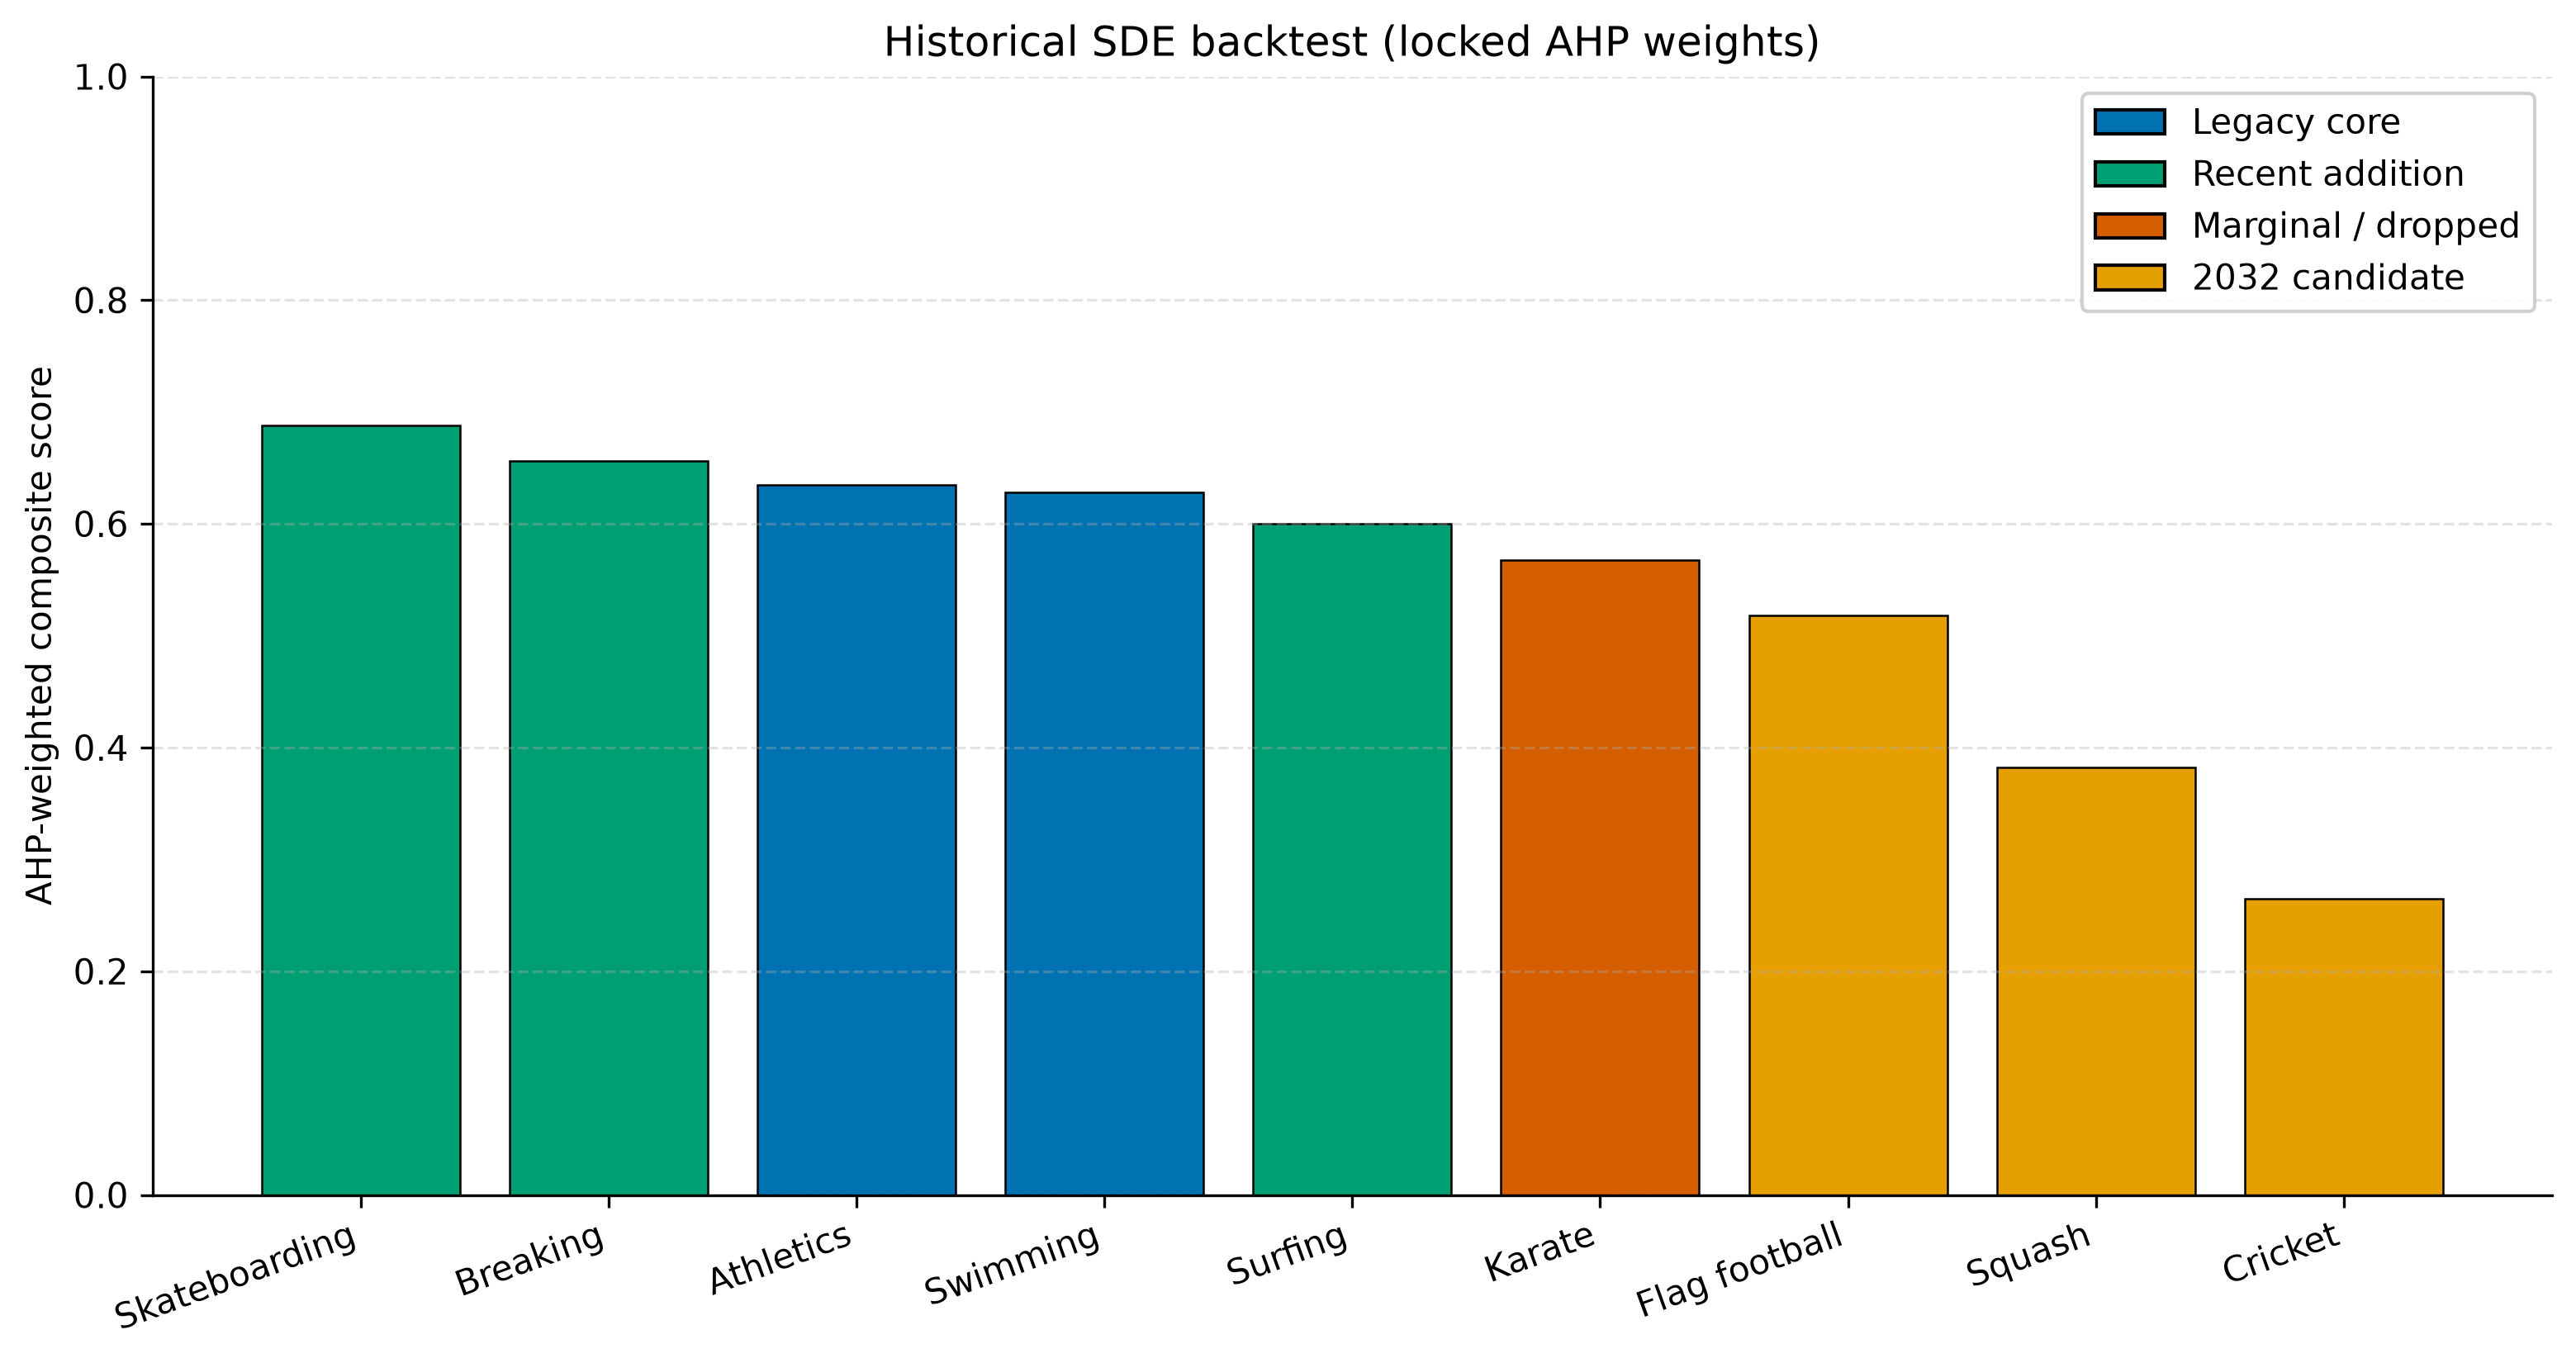
\includegraphics[width=0.92\textwidth]{fig_historical_backtest.png}
\caption{Locked-AHP historical back-test. Blue: legacy core; green: recent additions;
orange: marginal/exit; gold: 2032-tagged rows. Source:
\texttt{paper\_figures/fig\_historical\_backtest.png}.}
\label{fig:hist}
\end{figure}

\paragraph{Reading the back-test.}
Mean \(S_i\) of the three recent additions is \(0.6479\); the two legacy core sports
average \(0.6314\); Karate sits at \(0.5675\). High youth scores (9) and low
infrastructure cost (2--4) lift skateboarding and breaking above karate despite
karate's much larger federation reach (198). Athletics and swimming remain in the
top four because of appearances, reach, and broadcast, which is consistent with
their uninterrupted presence on the programme. The ordering is a directional check
against IOC youth-and-city decisions after 2020; it is not a causal proof, and the
three 2032-tagged rows in this table use the historical research leaves (for
example cricket gender \(42\) and youth \(5\)), not the later Brisbane scenario
file.

\section{Brisbane 2032 Forecast}
\label{sec:bris}

Table~\ref{tab:bris} is \texttt{results/brisbane\_2032\_ranking.csv}: the same
\(w\), but min-max taken only among Cricket, Squash, and Flag football, with the
Brisbane host-scenario leaves.

\begin{table}[htbp]
\centering
\caption{Brisbane 2032 three-candidate ranking from \texttt{brisbane\_2032\_ranking.csv}.}
\label{tab:bris}
\begin{tabular}{ll l rrrrr}
\toprule
Place & SDE & Role in script & Reach & Gender & Youth & Infra & \(S_i\) \\
\midrule
1st & Flag football & emerging youth & 75 & 50.0 & 8.5 & 3.5 & 0.5360 \\
2nd & Cricket & traditional host & 108 & 45.0 & 8.0 & 5.5 & 0.4842 \\
3rd & Squash & established niche & 150 & 48.0 & 6.5 & 3.0 & 0.3960 \\
\bottomrule
\end{tabular}
\end{table}

\paragraph{Why first: Flag football.}
It records the best gender share (\(50\)) and the best youth score (\(8.5\)) in the
trio, with a moderate infrastructure mark (\(3.5\)). Under a weight vector that
puts \(0.22\) on youth and \(0.16\) on gender, those leaves dominate the small
membership count (\(75\)).

\paragraph{Why second: Cricket.}
It is the only candidate with two recorded Olympic appearances in the workbook and
the strongest broadcast leaf (\(9.5\)). Reach (\(108\)) sits between the other two.
The model does \emph{not} add the stored host-popularity \(9.8\) into \(S_i\); any
``Brisbane loves cricket'' argument is extra-model.

\paragraph{Why third: Squash.}
It wins inclusivity (reach \(150\)) and has the lightest infrastructure score
(\(3.0\)), but the youth leaf (\(6.5\)) is the weakest of the three. With youth as
the largest AHP mass, that deficit is enough to finish last in the baseline.

These three \(S_i\) values are not comparable to Table~\ref{tab:hist}: the
normalization windows differ, and several Brisbane leaves differ from the historical
research file.

\subsection{Machine Learning Cross-Validation and Probability Prediction}
% Auto-generated by src/ml/plot_and_report.py --- do not hand-edit numbers.
% Source CSVs: results/ml_prediction_2032.csv, results/ahp_vs_ml_weights.csv
% Nested under \subsection{Machine Learning Cross-Validation and Probability Prediction}
\label{sec:ml-validation}

We treat the locked AHP--SAW ranking as a \emph{normative} score (what the team
values) and the L2 logistic model as a \emph{descriptive} inclusion probability
(what a tiny labelled history of stay-versus-exit can support). The two exercises
share the same six IOC leaves; the classifier also includes inertia features that
are dropped before comparing \(|\beta|\) with AHP. All figures and tables in this
section are written from \texttt{results/*.csv} by \texttt{src/ml/plot\_and\_report.py}.

\subsubsection{Leave-one-out diagnostics}

On the sourced labelled panel (\(N=6\): four stay cases and two one-Games exits)
leave-one-out logistic predictions yield
accuracy \(=0.3333\), ROC-AUC \(=0.5000\), and Brier score
\(=0.2475\) (Brier \(=\frac{1}{N}\sum_i(\hat p_i-y_i)^2\)).
A constant forecast \(\hat p=0.5\) has Brier \(0.25\); the observed Brier
\(0.2475\) is therefore close to an uninformative baseline.
This is \emph{not} high LOOCV accuracy, and it does not by itself prove that the
criterion list is statistically sufficient. What it does show, honestly, is that
with six rows and eight raw columns the inclusion model is a specification check:
useful for reading \(|\beta|\) against AHP, not for claiming a validated classifier.
The random-forest LOOCV AUC on the same split is even weaker, so we keep logistic
as the interpretable primary and AHP--SAW as the decision engine.

\subsubsection{Brisbane 2032 probabilities}

Table~\ref{tab:ml2032} copies \texttt{ml\_prediction\_2032.csv}.
Logistic bootstrap means (\(B=500\)) are Cricket \(0.7984\)
(95\% CI \(0.2689\)--\(0.9541\), tier
\texttt{high}),
Flag football \(0.6384\)
(\(0.1158\)--\(0.8994\),
\texttt{medium}),
and Squash \(0.4215\)
(\(0.1152\)--\(0.7042\),
\texttt{low}).
Figure~\ref{fig:ml2032} draws the same intervals and the \(P=0.50\) line.
Every interval still covers values both below and above one-half, so no candidate
is a statistically sharp ``in'' or ``out'' call.

\begin{table}[htbp]
\centering
\caption{2032 inclusion probabilities from \texttt{ml\_prediction\_2032.csv}
(logistic CI from bootstrap percentiles).}
\label{tab:ml2032}
\begin{tabular}{l r r r r l}
\toprule
SDE & \(P_{\mathrm{logit}}\) & \(P_{\mathrm{RF}}\) & CI low & CI high & tier \\
\midrule
Cricket & 0.7984 & 0.6535 & 0.2689 & 0.9541 & high \\
Squash & 0.4215 & 0.5913 & 0.1152 & 0.7042 & low \\
Flag football & 0.6384 & 0.6079 & 0.1158 & 0.8994 & medium \\
\bottomrule
\end{tabular}
\end{table}

\begin{figure}[htbp]
\centering
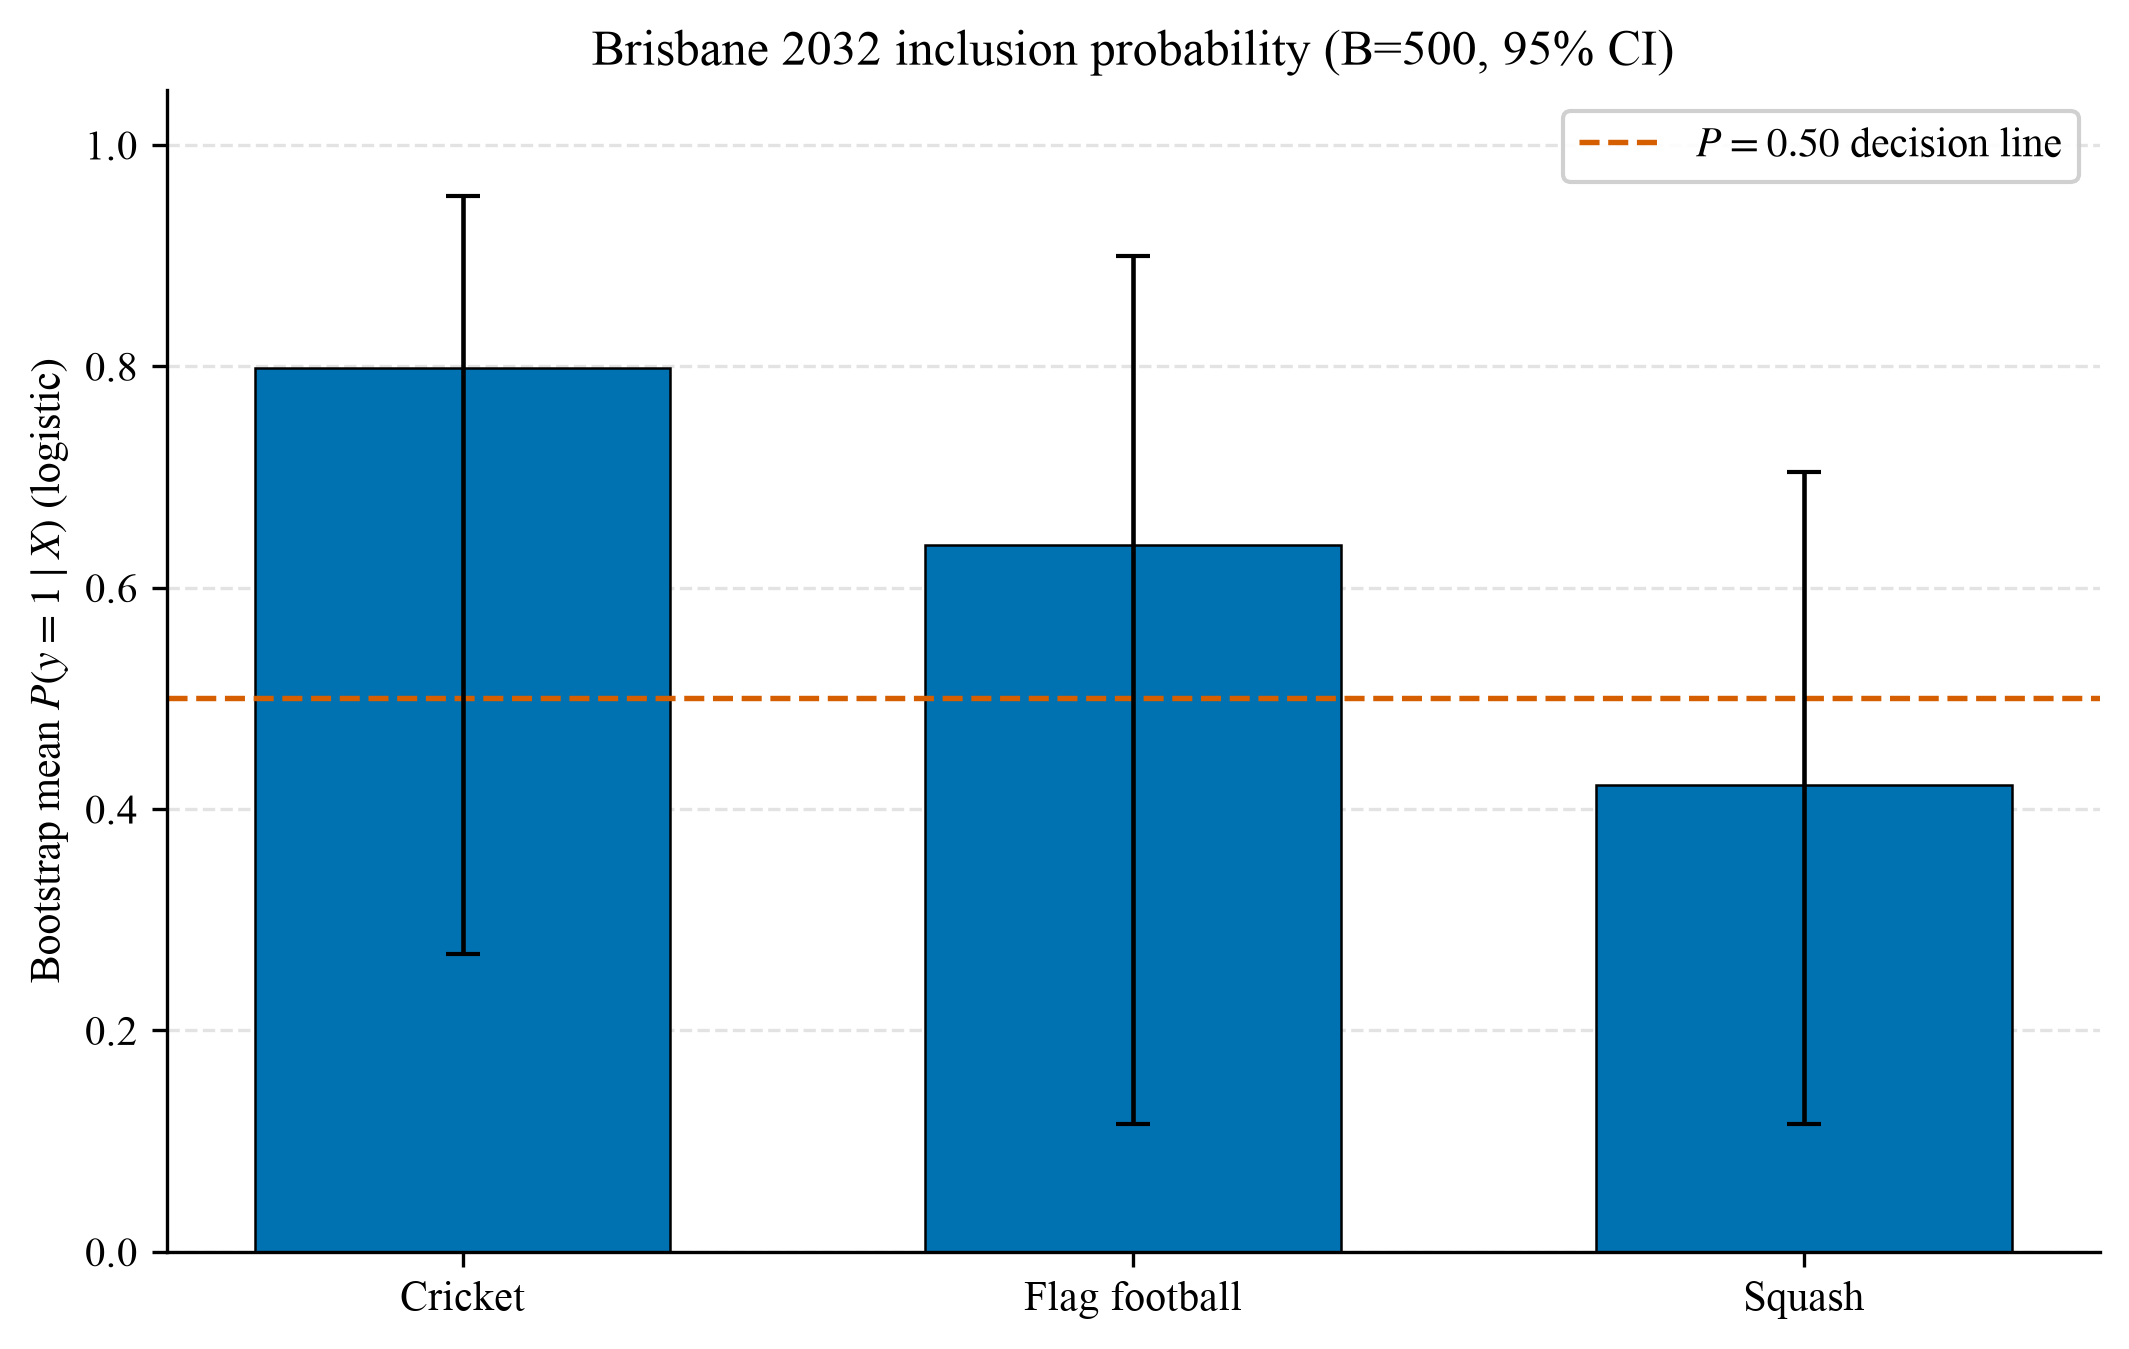
\includegraphics[width=0.88\textwidth]{fig_ml_2032_probability.png}
\caption{Logistic bootstrap means and 95\% intervals for Brisbane 2032 candidates.
Dashed line: \(P=0.50\). Source: \texttt{paper\_figures/fig\_ml\_2032\_probability.png}.}
\label{fig:ml2032}
\end{figure}

\subsubsection{AHP versus \(|\beta|\), and triangulation with SAW}

Table~\ref{tab:ahpml} and Figure~\ref{fig:dumbbell} compare L1-normalized
logistic \(|\beta|\) on the six IOC leaves with the locked AHP vector restricted
to the same six names. The largest positive gap
\(\Delta w = w^{\mathrm{ML}}-w^{\mathrm{AHP}}\) is
\texttt{BROADCAST\_VAL}
(\(\Delta w=0.2557\)):
the stay/exit labels put more mass on that leaf than the expert prior.
Youth appeal and gender parity go the other way---AHP is larger---and gender
has zero ML weight because all six labelled sports sit at a 50\% gender share.
The six-dimensional cosine between the two simplices is 0.7193.

Methodological triangulation is therefore only \emph{partial}.
AHP--SAW on the three-candidate universe ranks \textbf{Flag football}
first (composite \(0.5360\) in \texttt{brisbane\_2032\_ranking.csv}).
The logistic bootstrap mean instead ranks \textbf{Cricket} first.
Flag football remains in the SAW gold medal and in the ML \texttt{medium} tier,
so both paradigms keep it above Squash; they do not jointly lock a unique 2032
add. We report that tension rather than force a ``strict first-place lock.''
Programme advice stays with the AHP--SAW ranking and the youth-weight sensitivity
already stated; the classifier is a second lens, not a trump card.

\begin{table}[htbp]
\centering
\caption{Six-criterion AHP versus logistic \(|\beta|\) from
\texttt{ahp\_vs\_ml\_weights.csv}. Difference \(=w^{\mathrm{ML}}-w^{\mathrm{AHP}}\).}
\label{tab:ahpml}
\begin{tabular}{l r r r l}
\toprule
Criterion & AHP & ML & \(\Delta w\) & reading \\
\midrule
GLOBAL\_REACH & 0.2000 & 0.1295 & -0.0705 & AHP\_higher\_than\_ML \\
GENDER\_PARITY & 0.1778 & 0.0000 & -0.1778 & AHP\_higher\_than\_ML \\
YOUTH\_APPEAL & 0.2444 & 0.1285 & -0.1159 & AHP\_higher\_than\_ML \\
INFRA\_COST & 0.1333 & 0.2813 & 0.1480 & ML\_higher\_than\_AHP \\
BROADCAST\_VAL & 0.1556 & 0.4113 & 0.2557 & ML\_higher\_than\_AHP \\
Events\_Count & 0.0889 & 0.0494 & -0.0395 & AHP\_higher\_than\_ML \\
\bottomrule
\end{tabular}
\end{table}

\begin{figure}[htbp]
\centering
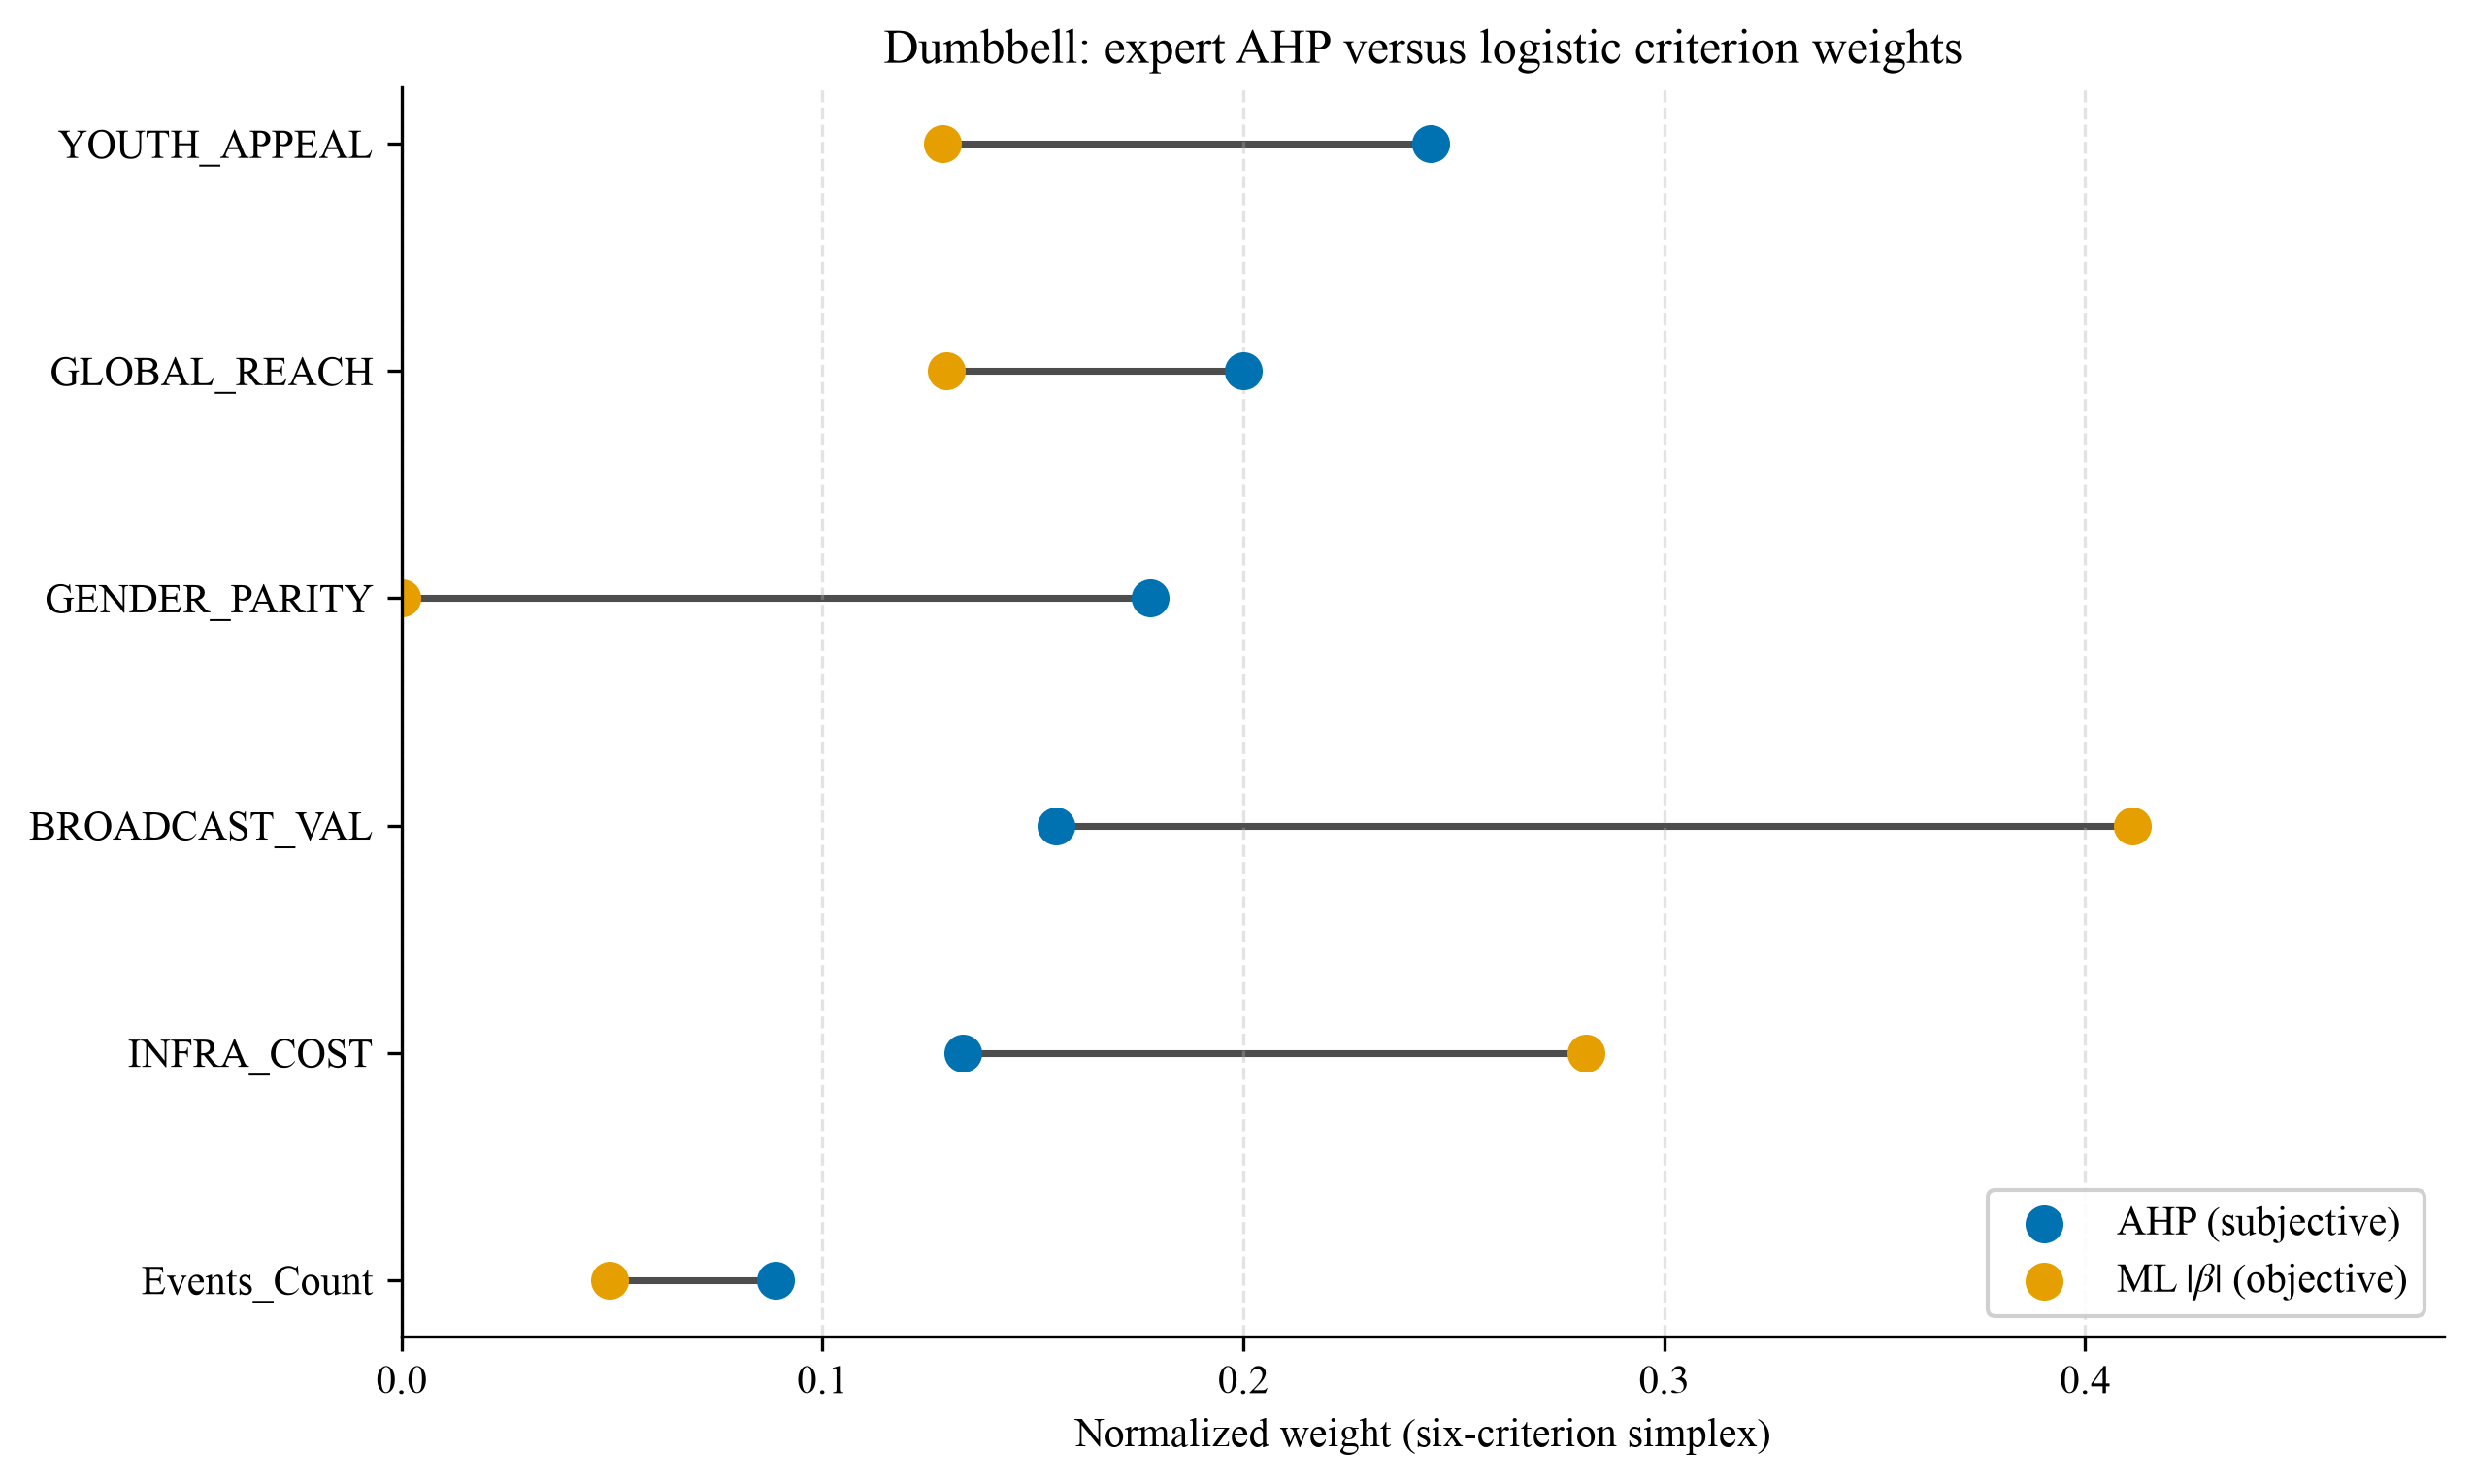
\includegraphics[width=0.92\textwidth]{fig_ahp_vs_ml_dumbbell.png}
\caption{Dumbbell plot of subjective AHP weights (blue) and objective logistic
weights (orange). Source: \texttt{paper\_figures/fig\_ahp\_vs\_ml\_dumbbell.png}.}
\label{fig:dumbbell}
\end{figure}


\section{Sensitivity and Robustness Analysis}
\label{sec:sens}

One-at-a-time shocks multiply every leaf in an IOC group by \(1.20\) or \(0.80\) and
renormalize \(w\) to a probability vector. Groups are Popularity/Accessibility
(Appearances and BROADCAST\_VAL), Programme footprint (Events\_Count), Inclusivity,
Gender equity, Relevance/Innovation (YOUTH\_APPEAL), and Sustainability. An extra
extreme case sets the youth weight to zero and renormalizes the rest.

Table~\ref{tab:oat} compresses \texttt{results/sensitivity\_weight\_shock.csv} for
the Brisbane universe. Every \(\pm 20\%\) row keeps Flag football--Cricket--Squash as
1--2--3. Cricket's rank never leaves second place in that universe (rank range \(0\)
across 14 scenarios). Flag football is first in 13 of 14 scenarios and third when
youth is removed.

\begin{table}[htbp]
\centering
\caption{Brisbane-universe ranks under locked weights, every \(\pm 20\%\) OAT group
(all identical), and youth weight \(=0\). Source: \texttt{sensitivity\_weight\_shock.csv}.}
\label{tab:oat}
\begin{tabular}{l ccc}
\toprule
SDE & Baseline / all \(\pm 20\%\) & Youth \(=0\) & \(\Delta\) rank at youth \(=0\) \\
\midrule
Flag football & 1st (\(S=0.5360\)) & 3rd (\(S=0.4051\)) & \(-2\) \\
Cricket       & 2nd (\(S=0.4842\)) & 2nd (\(S=0.4092\)) & \(0\) \\
Squash        & 3rd (\(S=0.3960\)) & 1st (\(S=0.5077\)) & \(+2\) \\
\bottomrule
\end{tabular}
\end{table}

On the nine-row \texttt{sde\_matrix} universe the same youth-zero experiment
reorders core versus urban sports (Table~\ref{tab:youth9}).

\begin{table}[htbp]
\centering
\caption{Selected ranks on the nine-row matrix, baseline versus youth weight \(=0\).}
\label{tab:youth9}
\begin{tabular}{l cc}
\toprule
SDE & Baseline rank & Rank after youth \(=0\) \\
\midrule
Skateboarding & 1 & 4 \\
Breaking      & 2 & 8 \\
Flag football & 3 & 6 \\
Athletics     & 4 & 1 \\
Surfing       & 5 & 7 \\
Swimming      & 6 & 2 \\
Karate        & 7 & 3 \\
Cricket       & 8 & 9 \\
Squash        & 9 & 5 \\
\bottomrule
\end{tabular}
\end{table}

Figure~\ref{fig:sens} shows the Brisbane score and rank walks. The practical
conclusion is sharp: the 2032 medal order is \emph{locally} robust to twenty-percent
criterion noise and \emph{globally} fragile to dropping youth appeal. A decision
maker who does not accept a \(0.22\) youth weight should not adopt Flag football as
an automatic first pick; Squash then leads the trio, and Athletics/Swimming lead the
nine-sport panel.

\begin{figure}[htbp]
\centering
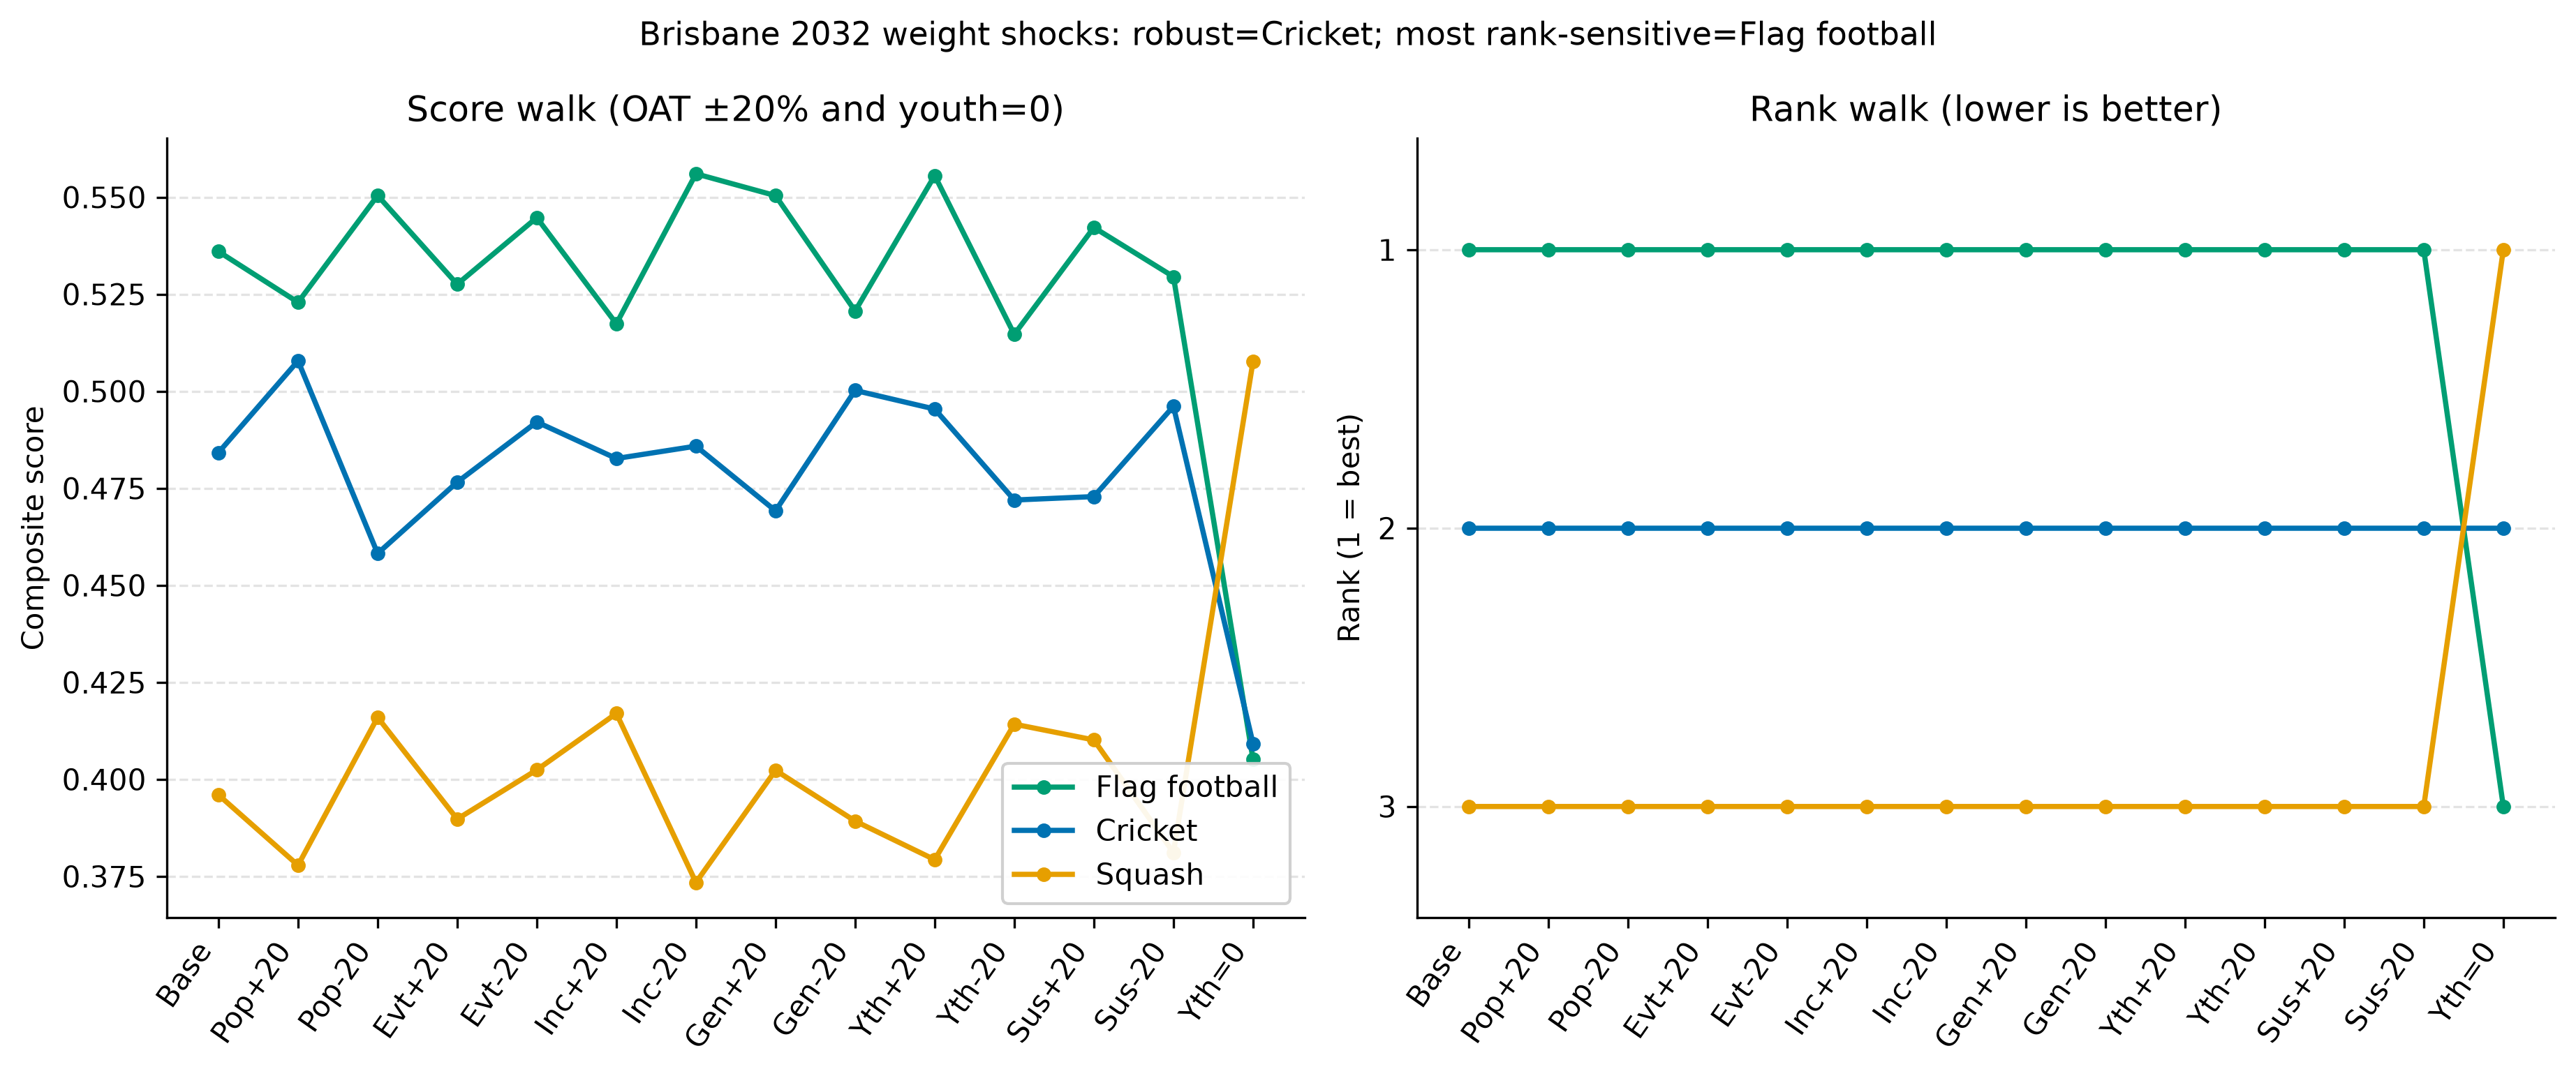
\includegraphics[width=0.98\textwidth]{fig_sensitivity_shock.png}
\caption{Parallel-coordinate shock plot from
\texttt{paper\_figures/fig\_sensitivity\_shock.png}. Left: composite scores; right:
ranks (1 at the top). The only rank crossing among the three candidates is the
youth-zero scenario.}
\label{fig:sens}
\end{figure}

\section{Strengths and Limitations}
\label{sec:lim}

\paragraph{Strengths.}
The comparison matrix is algebraically consistent (\(\CR=0\)), so rank discussion is
not confounded by Saaty inconsistency. Leaves have an explicit benefit/cost sense
and a documented source split (xlsx versus research CSV versus Brisbane scenario).
Historical and 2032 runs share one weight vector. Sensitivity is a full OAT table
written to disk, not a narrative claim.

\paragraph{Subjective weights.}
Locking \(w\) from a team prior is still a value judgement. Ratio construction
hides disagreement that a filled 1--9 questionnaire would have revealed. The
youth-zero case shows that this judgement is decisive.

\paragraph{Scale and rank reversal.}
Min-max depends on the alternative set. Adding or deleting an SDE can reorder the
others (a known SAW/AHP rank-reversal issue). That is why Table~\ref{tab:hist} and
Table~\ref{tab:bris} are reported separately.

\paragraph{Missing IOC content.}
Fairness, anti-doping, athlete numbers, and domestic broadcast rights in Australia
are not columns. \texttt{HOST\_POPULARITY} exists for the three candidates and is
omitted from \(S_i\) by design; including it would require a new eighth weight and a
new locked matrix.

\paragraph{Data grain.}
Federation membership is a coarse proxy for inclusivity. Gender shares of \(50\)
are Paris-parity defaults, not event-by-event starts. Saaty leaves are research
scores, not ticket or TV measurements. Cricket's historical-panel gender \(42\) and
Brisbane-scenario gender \(45\) already show that two honest tables need not match.

\paragraph{What we would do next.}
Re-elicit \(A\) from several independent pairwise matrices and take a geometric
mean; add a TOPSIS ranking already implemented in code as a cross-check; put host
popularity into a second-stage AHP only after a new consistency test; and replace
Saaty broadcast scores with audited rights-fee or audience figures if they become
available.

\section*{References}

\begin{enumerate}
\item T.~L.~Saaty, \emph{The Analytic Hierarchy Process}. McGraw-Hill, 1980.
\item International Olympic Committee, Olympic Agenda 2020 and related programme
      documentation (public IOC materials on youth, gender parity, and sustainability).
\item COMAP, HiMCM 2024 Problem A data workbook \texttt{HiMCM\_Olympic\_Data.xlsx}.
\item Kardi Teknomo, \emph{Analytic Hierarchy Process (AHP) Tutorial} (notes on
      eigenvalue weights, \(\CR\), and the danger of mixing units before weighting).
\item Team files: \texttt{results/historical\_ranking.csv},
      \texttt{results/brisbane\_2032\_ranking.csv},
      \texttt{results/sensitivity\_weight\_shock.csv}.
\end{enumerate}

\end{document}
